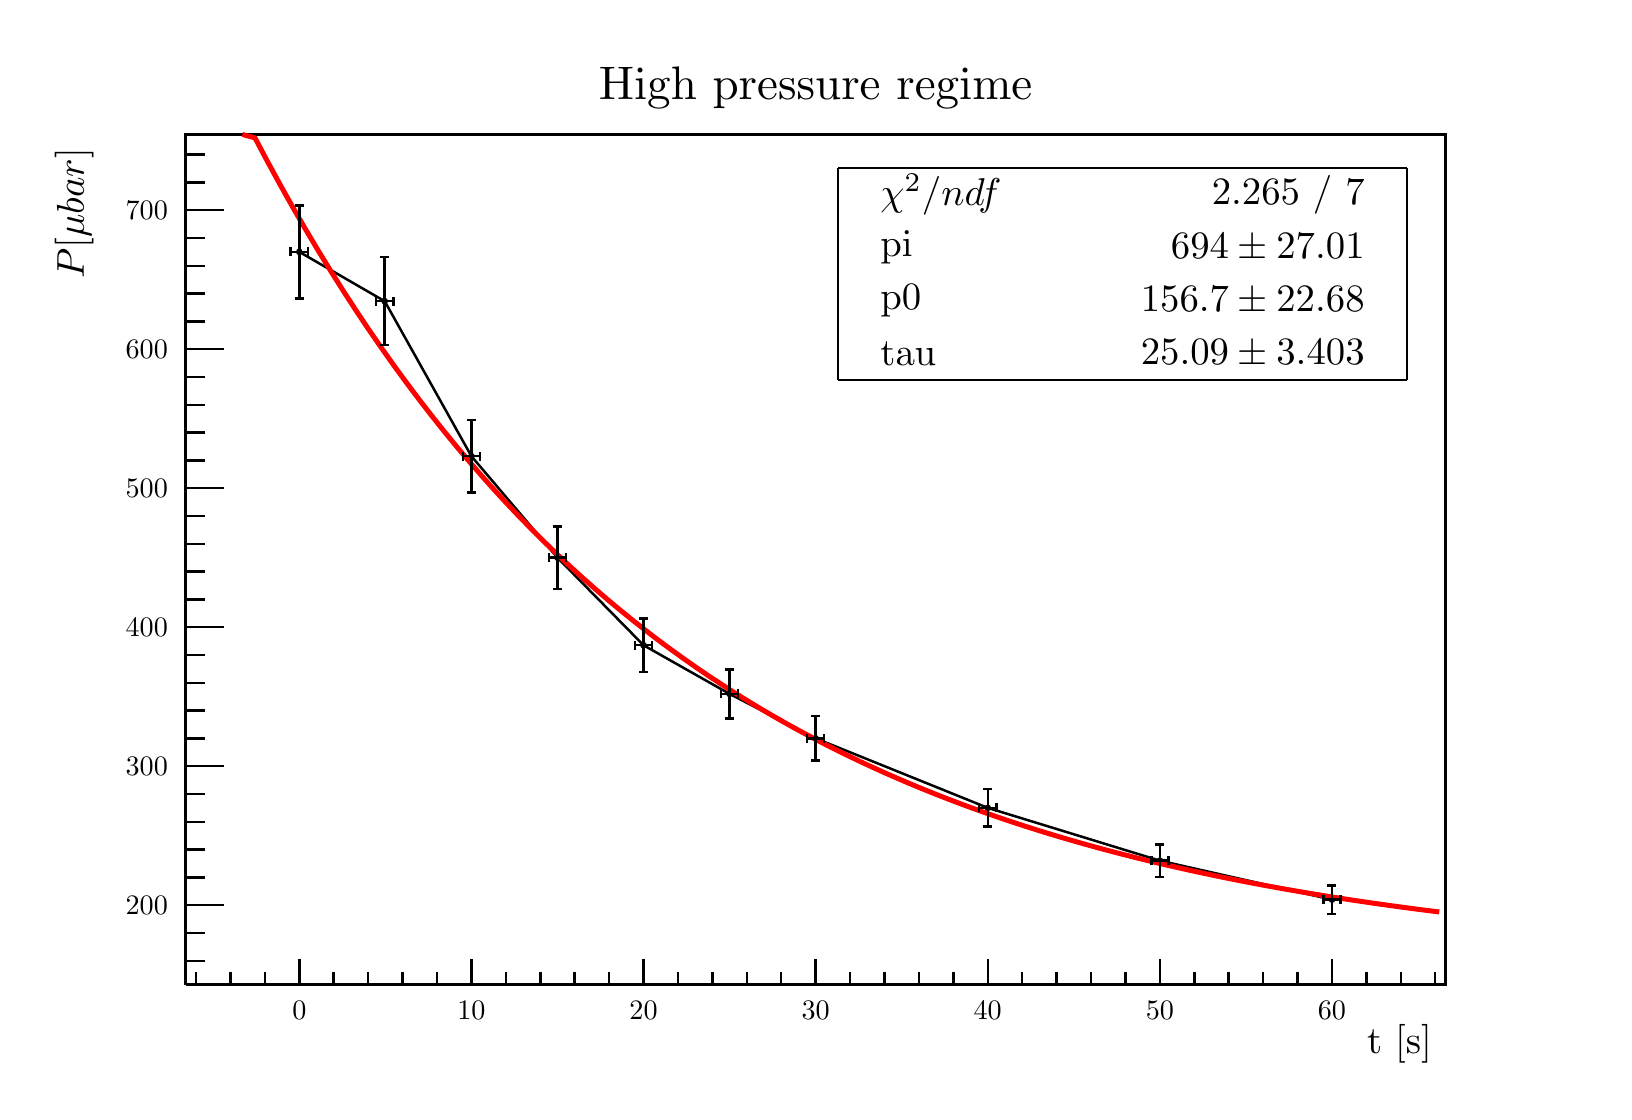
\begin{tikzpicture}
\pgfdeclareplotmark{cross} {
\pgfpathmoveto{\pgfpoint{-0.3\pgfplotmarksize}{\pgfplotmarksize}}
\pgfpathlineto{\pgfpoint{+0.3\pgfplotmarksize}{\pgfplotmarksize}}
\pgfpathlineto{\pgfpoint{+0.3\pgfplotmarksize}{0.3\pgfplotmarksize}}
\pgfpathlineto{\pgfpoint{+1\pgfplotmarksize}{0.3\pgfplotmarksize}}
\pgfpathlineto{\pgfpoint{+1\pgfplotmarksize}{-0.3\pgfplotmarksize}}
\pgfpathlineto{\pgfpoint{+0.3\pgfplotmarksize}{-0.3\pgfplotmarksize}}
\pgfpathlineto{\pgfpoint{+0.3\pgfplotmarksize}{-1.\pgfplotmarksize}}
\pgfpathlineto{\pgfpoint{-0.3\pgfplotmarksize}{-1.\pgfplotmarksize}}
\pgfpathlineto{\pgfpoint{-0.3\pgfplotmarksize}{-0.3\pgfplotmarksize}}
\pgfpathlineto{\pgfpoint{-1.\pgfplotmarksize}{-0.3\pgfplotmarksize}}
\pgfpathlineto{\pgfpoint{-1.\pgfplotmarksize}{0.3\pgfplotmarksize}}
\pgfpathlineto{\pgfpoint{-0.3\pgfplotmarksize}{0.3\pgfplotmarksize}}
\pgfpathclose
\pgfusepathqstroke
}
\pgfdeclareplotmark{cross*} {
\pgfpathmoveto{\pgfpoint{-0.3\pgfplotmarksize}{\pgfplotmarksize}}
\pgfpathlineto{\pgfpoint{+0.3\pgfplotmarksize}{\pgfplotmarksize}}
\pgfpathlineto{\pgfpoint{+0.3\pgfplotmarksize}{0.3\pgfplotmarksize}}
\pgfpathlineto{\pgfpoint{+1\pgfplotmarksize}{0.3\pgfplotmarksize}}
\pgfpathlineto{\pgfpoint{+1\pgfplotmarksize}{-0.3\pgfplotmarksize}}
\pgfpathlineto{\pgfpoint{+0.3\pgfplotmarksize}{-0.3\pgfplotmarksize}}
\pgfpathlineto{\pgfpoint{+0.3\pgfplotmarksize}{-1.\pgfplotmarksize}}
\pgfpathlineto{\pgfpoint{-0.3\pgfplotmarksize}{-1.\pgfplotmarksize}}
\pgfpathlineto{\pgfpoint{-0.3\pgfplotmarksize}{-0.3\pgfplotmarksize}}
\pgfpathlineto{\pgfpoint{-1.\pgfplotmarksize}{-0.3\pgfplotmarksize}}
\pgfpathlineto{\pgfpoint{-1.\pgfplotmarksize}{0.3\pgfplotmarksize}}
\pgfpathlineto{\pgfpoint{-0.3\pgfplotmarksize}{0.3\pgfplotmarksize}}
\pgfpathclose
\pgfusepathqfillstroke
}
\pgfdeclareplotmark{newstar} {
\pgfpathmoveto{\pgfqpoint{0pt}{\pgfplotmarksize}}
\pgfpathlineto{\pgfqpointpolar{44}{0.5\pgfplotmarksize}}
\pgfpathlineto{\pgfqpointpolar{18}{\pgfplotmarksize}}
\pgfpathlineto{\pgfqpointpolar{-20}{0.5\pgfplotmarksize}}
\pgfpathlineto{\pgfqpointpolar{-54}{\pgfplotmarksize}}
\pgfpathlineto{\pgfqpointpolar{-90}{0.5\pgfplotmarksize}}
\pgfpathlineto{\pgfqpointpolar{234}{\pgfplotmarksize}}
\pgfpathlineto{\pgfqpointpolar{198}{0.5\pgfplotmarksize}}
\pgfpathlineto{\pgfqpointpolar{162}{\pgfplotmarksize}}
\pgfpathlineto{\pgfqpointpolar{134}{0.5\pgfplotmarksize}}
\pgfpathclose
\pgfusepathqstroke
}
\pgfdeclareplotmark{newstar*} {
\pgfpathmoveto{\pgfqpoint{0pt}{\pgfplotmarksize}}
\pgfpathlineto{\pgfqpointpolar{44}{0.5\pgfplotmarksize}}
\pgfpathlineto{\pgfqpointpolar{18}{\pgfplotmarksize}}
\pgfpathlineto{\pgfqpointpolar{-20}{0.5\pgfplotmarksize}}
\pgfpathlineto{\pgfqpointpolar{-54}{\pgfplotmarksize}}
\pgfpathlineto{\pgfqpointpolar{-90}{0.5\pgfplotmarksize}}
\pgfpathlineto{\pgfqpointpolar{234}{\pgfplotmarksize}}
\pgfpathlineto{\pgfqpointpolar{198}{0.5\pgfplotmarksize}}
\pgfpathlineto{\pgfqpointpolar{162}{\pgfplotmarksize}}
\pgfpathlineto{\pgfqpointpolar{134}{0.5\pgfplotmarksize}}
\pgfpathclose
\pgfusepathqfillstroke
}
\definecolor{c}{rgb}{1,1,1};
\draw [color=c, fill=c] (0,0) rectangle (20,13.4957);
\draw [color=c, fill=c] (2,1.34957) rectangle (18,12.1461);
\definecolor{c}{rgb}{0,0,0};
\draw [c,line width=0.9] (2,1.34957) -- (2,12.1461) -- (18,12.1461) -- (18,1.34957) -- (2,1.34957);
\definecolor{c}{rgb}{1,1,1};
\draw [color=c, fill=c] (2,1.34957) rectangle (18,12.1461);
\definecolor{c}{rgb}{0,0,0};
\draw [c,line width=0.9] (2,1.34957) -- (2,12.1461) -- (18,12.1461) -- (18,1.34957) -- (2,1.34957);
\draw [c,line width=0.9] (2,1.34957) -- (18,1.34957);
\draw [c,line width=0.9] (3.44262,1.67347) -- (3.44262,1.34957);
\draw [c,line width=0.9] (3.87978,1.51152) -- (3.87978,1.34957);
\draw [c,line width=0.9] (4.31694,1.51152) -- (4.31694,1.34957);
\draw [c,line width=0.9] (4.7541,1.51152) -- (4.7541,1.34957);
\draw [c,line width=0.9] (5.19126,1.51152) -- (5.19126,1.34957);
\draw [c,line width=0.9] (5.62842,1.67347) -- (5.62842,1.34957);
\draw [c,line width=0.9] (6.06557,1.51152) -- (6.06557,1.34957);
\draw [c,line width=0.9] (6.50273,1.51152) -- (6.50273,1.34957);
\draw [c,line width=0.9] (6.93989,1.51152) -- (6.93989,1.34957);
\draw [c,line width=0.9] (7.37705,1.51152) -- (7.37705,1.34957);
\draw [c,line width=0.9] (7.81421,1.67347) -- (7.81421,1.34957);
\draw [c,line width=0.9] (8.25137,1.51152) -- (8.25137,1.34957);
\draw [c,line width=0.9] (8.68852,1.51152) -- (8.68852,1.34957);
\draw [c,line width=0.9] (9.12568,1.51152) -- (9.12568,1.34957);
\draw [c,line width=0.9] (9.56284,1.51152) -- (9.56284,1.34957);
\draw [c,line width=0.9] (10,1.67347) -- (10,1.34957);
\draw [c,line width=0.9] (10.4372,1.51152) -- (10.4372,1.34957);
\draw [c,line width=0.9] (10.8743,1.51152) -- (10.8743,1.34957);
\draw [c,line width=0.9] (11.3115,1.51152) -- (11.3115,1.34957);
\draw [c,line width=0.9] (11.7486,1.51152) -- (11.7486,1.34957);
\draw [c,line width=0.9] (12.1858,1.67347) -- (12.1858,1.34957);
\draw [c,line width=0.9] (12.623,1.51152) -- (12.623,1.34957);
\draw [c,line width=0.9] (13.0601,1.51152) -- (13.0601,1.34957);
\draw [c,line width=0.9] (13.4973,1.51152) -- (13.4973,1.34957);
\draw [c,line width=0.9] (13.9344,1.51152) -- (13.9344,1.34957);
\draw [c,line width=0.9] (14.3716,1.67347) -- (14.3716,1.34957);
\draw [c,line width=0.9] (14.8087,1.51152) -- (14.8087,1.34957);
\draw [c,line width=0.9] (15.2459,1.51152) -- (15.2459,1.34957);
\draw [c,line width=0.9] (15.6831,1.51152) -- (15.6831,1.34957);
\draw [c,line width=0.9] (16.1202,1.51152) -- (16.1202,1.34957);
\draw [c,line width=0.9] (16.5574,1.67347) -- (16.5574,1.34957);
\draw [c,line width=0.9] (3.44262,1.67347) -- (3.44262,1.34957);
\draw [c,line width=0.9] (3.00546,1.51152) -- (3.00546,1.34957);
\draw [c,line width=0.9] (2.56831,1.51152) -- (2.56831,1.34957);
\draw [c,line width=0.9] (2.13115,1.51152) -- (2.13115,1.34957);
\draw [c,line width=0.9] (16.5574,1.67347) -- (16.5574,1.34957);
\draw [c,line width=0.9] (16.9945,1.51152) -- (16.9945,1.34957);
\draw [c,line width=0.9] (17.4317,1.51152) -- (17.4317,1.34957);
\draw [c,line width=0.9] (17.8689,1.51152) -- (17.8689,1.34957);
\draw [anchor=base] (3.44262,0.904212) node[scale=1.01821, color=c, rotate=0]{0};
\draw [anchor=base] (5.62842,0.904212) node[scale=1.01821, color=c, rotate=0]{10};
\draw [anchor=base] (7.81421,0.904212) node[scale=1.01821, color=c, rotate=0]{20};
\draw [anchor=base] (10,0.904212) node[scale=1.01821, color=c, rotate=0]{30};
\draw [anchor=base] (12.1858,0.904212) node[scale=1.01821, color=c, rotate=0]{40};
\draw [anchor=base] (14.3716,0.904212) node[scale=1.01821, color=c, rotate=0]{50};
\draw [anchor=base] (16.5574,0.904212) node[scale=1.01821, color=c, rotate=0]{60};
\draw [anchor= east] (18,0.593811) node[scale=1.4, color=c, rotate=0]{t [s]};
\draw [c,line width=0.9] (2,1.34957) -- (2,12.1461);
\draw [c,line width=0.9] (2.48,2.35873) -- (2,2.35873);
\draw [c,line width=0.9] (2.24,2.71176) -- (2,2.71176);
\draw [c,line width=0.9] (2.24,3.0648) -- (2,3.0648);
\draw [c,line width=0.9] (2.24,3.41783) -- (2,3.41783);
\draw [c,line width=0.9] (2.24,3.77087) -- (2,3.77087);
\draw [c,line width=0.9] (2.48,4.12391) -- (2,4.12391);
\draw [c,line width=0.9] (2.24,4.47694) -- (2,4.47694);
\draw [c,line width=0.9] (2.24,4.82998) -- (2,4.82998);
\draw [c,line width=0.9] (2.24,5.18302) -- (2,5.18302);
\draw [c,line width=0.9] (2.24,5.53605) -- (2,5.53605);
\draw [c,line width=0.9] (2.48,5.88909) -- (2,5.88909);
\draw [c,line width=0.9] (2.24,6.24213) -- (2,6.24213);
\draw [c,line width=0.9] (2.24,6.59516) -- (2,6.59516);
\draw [c,line width=0.9] (2.24,6.9482) -- (2,6.9482);
\draw [c,line width=0.9] (2.24,7.30124) -- (2,7.30124);
\draw [c,line width=0.9] (2.48,7.65427) -- (2,7.65427);
\draw [c,line width=0.9] (2.24,8.00731) -- (2,8.00731);
\draw [c,line width=0.9] (2.24,8.36034) -- (2,8.36034);
\draw [c,line width=0.9] (2.24,8.71338) -- (2,8.71338);
\draw [c,line width=0.9] (2.24,9.06642) -- (2,9.06642);
\draw [c,line width=0.9] (2.48,9.41945) -- (2,9.41945);
\draw [c,line width=0.9] (2.24,9.77249) -- (2,9.77249);
\draw [c,line width=0.9] (2.24,10.1255) -- (2,10.1255);
\draw [c,line width=0.9] (2.24,10.4786) -- (2,10.4786);
\draw [c,line width=0.9] (2.24,10.8316) -- (2,10.8316);
\draw [c,line width=0.9] (2.48,11.1846) -- (2,11.1846);
\draw [c,line width=0.9] (2.48,2.35873) -- (2,2.35873);
\draw [c,line width=0.9] (2.24,2.00569) -- (2,2.00569);
\draw [c,line width=0.9] (2.24,1.65265) -- (2,1.65265);
\draw [c,line width=0.9] (2.48,11.1846) -- (2,11.1846);
\draw [c,line width=0.9] (2.24,11.5377) -- (2,11.5377);
\draw [c,line width=0.9] (2.24,11.8907) -- (2,11.8907);
\draw [anchor= east] (1.9,2.35873) node[scale=1.01821, color=c, rotate=0]{200};
\draw [anchor= east] (1.9,4.12391) node[scale=1.01821, color=c, rotate=0]{300};
\draw [anchor= east] (1.9,5.88909) node[scale=1.01821, color=c, rotate=0]{400};
\draw [anchor= east] (1.9,7.65427) node[scale=1.01821, color=c, rotate=0]{500};
\draw [anchor= east] (1.9,9.41945) node[scale=1.01821, color=c, rotate=0]{600};
\draw [anchor= east] (1.9,11.1846) node[scale=1.01821, color=c, rotate=0]{700};
\draw [anchor= east] (0.583668,12.1461) node[scale=1.4, color=c, rotate=90]{$P [\mu bar]$};
\draw [c,line width=0.9] (3.44262,10.6551) -- (4.52722,10.0287) -- (5.62842,8.06026) -- (6.72131,6.77168) -- (7.81421,5.65962) -- (8.9071,5.0418) -- (10,4.47694) -- (12.1858,3.59435) -- (14.3716,2.92358) -- (16.5574,2.42933);
\foreach \P in {(3.44262,10.6551), (4.52722,10.0287), (5.62842,8.06026), (6.72131,6.77168), (7.81421,5.65962), (8.9071,5.0418), (10,4.47694), (12.1858,3.59435), (14.3716,2.92358), (16.5574,2.42933)}{\draw[mark options={color=c,fill=c},mark
 size=2.402402pt,mark=*,mark size=1pt] plot coordinates {\P};}
\definecolor{c}{rgb}{1,0,0};
\draw [c,line width=1.8] (2.72,12.1461) -- (2.88,12.1024) -- (3.04,11.8003) -- (3.2,11.5069) -- (3.36,11.2219) -- (3.52,10.9452) -- (3.68,10.6763) -- (3.84,10.4152) -- (4,10.1617) -- (4.16,9.91535) -- (4.32,9.67613) -- (4.48,9.44379) --
 (4.64,9.21813) -- (4.8,8.99896) -- (4.96,8.78609) -- (5.12,8.57934) -- (5.28,8.37853) -- (5.44,8.1835) -- (5.6,7.99408) -- (5.76,7.8101) -- (5.92,7.63141) -- (6.08,7.45786) -- (6.24,7.2893) -- (6.4,7.12558) -- (6.56,6.96657) -- (6.72,6.81214) --
 (6.88,6.66214) -- (7.04,6.51646) -- (7.2,6.37496) -- (7.36,6.23753) -- (7.52,6.10406) -- (7.68,5.97442) -- (7.84,5.84851) -- (8,5.72622) -- (8.16,5.60744) -- (8.32,5.49208) -- (8.48,5.38004) -- (8.64,5.27122) -- (8.8,5.16553) -- (8.96,5.06287) --
 (9.12,4.96317) -- (9.28,4.86633) -- (9.44,4.77228) -- (9.6,4.68093) -- (9.76,4.59221) -- (9.92,4.50604) -- (10.08,4.42235) -- (10.24,4.34106) -- (10.4,4.26211) -- (10.56,4.18543);
\draw [c,line width=1.8] (10.56,4.18543) -- (10.72,4.11096) -- (10.88,4.03862) -- (11.04,3.96837) -- (11.2,3.90013) -- (11.36,3.83386) -- (11.52,3.76949) -- (11.68,3.70698) -- (11.84,3.64626) -- (12,3.58729) -- (12.16,3.53001) -- (12.32,3.47438) --
 (12.48,3.42035) -- (12.64,3.36787) -- (12.8,3.3169) -- (12.96,3.2674) -- (13.12,3.21932) -- (13.28,3.17262) -- (13.44,3.12726) -- (13.6,3.08321) -- (13.76,3.04043) -- (13.92,2.99887) -- (14.08,2.95851) -- (14.24,2.91931) -- (14.4,2.88124) --
 (14.56,2.84426) -- (14.72,2.80835) -- (14.88,2.77346) -- (15.04,2.73958) -- (15.2,2.70668) -- (15.36,2.67472) -- (15.52,2.64368) -- (15.68,2.61353) -- (15.84,2.58425) -- (16,2.55581) -- (16.16,2.52819) -- (16.32,2.50136) -- (16.48,2.47531) --
 (16.64,2.45) -- (16.8,2.42542) -- (16.96,2.40155) -- (17.12,2.37836) -- (17.28,2.35584) -- (17.44,2.33397) -- (17.6,2.31273) -- (17.76,2.2921) -- (17.92,2.27206);
\definecolor{c}{rgb}{1,1,1};
\draw [color=c, fill=c] (10.2865,9.02579) rectangle (17.5072,11.7192);
\definecolor{c}{rgb}{0,0,0};
\draw [c,line width=0.9] (10.2865,9.02579) -- (17.5072,9.02579);
\draw [c,line width=0.9] (17.5072,9.02579) -- (17.5072,11.7192);
\draw [c,line width=0.9] (17.5072,11.7192) -- (10.2865,11.7192);
\draw [c,line width=0.9] (10.2865,11.7192) -- (10.2865,9.02579);
\draw [anchor= west] (10.6476,11.3825) node[scale=1.40004, color=c, rotate=0]{$\chi^{2} / ndf $};
\draw [anchor= east] (17.1461,11.3825) node[scale=1.40004, color=c, rotate=0]{ 2.265 / 7};
\draw [anchor= west] (10.6476,10.7092) node[scale=1.40004, color=c, rotate=0]{pi       };
\draw [anchor= east] (17.1461,10.7092) node[scale=1.40004, color=c, rotate=0]{$   694 \pm 27.01$};
\draw [anchor= west] (10.6476,10.0358) node[scale=1.40004, color=c, rotate=0]{p0       };
\draw [anchor= east] (17.1461,10.0358) node[scale=1.40004, color=c, rotate=0]{$ 156.7 \pm 22.68$};
\draw [anchor= west] (10.6476,9.36246) node[scale=1.40004, color=c, rotate=0]{tau      };
\draw [anchor= east] (17.1461,9.36246) node[scale=1.40004, color=c, rotate=0]{$ 25.09 \pm 3.403$};
\draw [c,line width=0.9] (3.44262,10.6551) -- (3.33333,10.6551);
\draw [c,line width=0.9] (3.33333,10.5978) -- (3.33333,10.7124);
\draw [c,line width=0.9] (3.44262,10.6551) -- (3.55191,10.6551);
\draw [c,line width=0.9] (3.55191,10.5978) -- (3.55191,10.7124);
\draw [c,line width=0.9] (3.44262,10.6551) -- (3.44262,11.2464);
\draw [c,line width=0.9] (3.38532,11.2464) -- (3.49993,11.2464);
\draw [c,line width=0.9] (3.44262,10.6551) -- (3.44262,10.0637);
\draw [c,line width=0.9] (3.38532,10.0637) -- (3.49993,10.0637);
\draw [c,line width=0.9] (4.52722,10.0287) -- (4.41793,10.0287);
\draw [c,line width=0.9] (4.41793,9.97135) -- (4.41793,10.086);
\draw [c,line width=0.9] (4.52722,10.0287) -- (4.63651,10.0287);
\draw [c,line width=0.9] (4.63651,9.97135) -- (4.63651,10.086);
\draw [c,line width=0.9] (4.52722,10.0287) -- (4.52722,10.5873);
\draw [c,line width=0.9] (4.46991,10.5873) -- (4.58453,10.5873);
\draw [c,line width=0.9] (4.52722,10.0287) -- (4.52722,9.46997);
\draw [c,line width=0.9] (4.46991,9.46997) -- (4.58453,9.46997);
\draw [c,line width=0.9] (5.62842,8.06026) -- (5.51913,8.06026);
\draw [c,line width=0.9] (5.51913,8.00296) -- (5.51913,8.11757);
\draw [c,line width=0.9] (5.62842,8.06026) -- (5.73771,8.06026);
\draw [c,line width=0.9] (5.73771,8.00296) -- (5.73771,8.11757);
\draw [c,line width=0.9] (5.62842,8.06026) -- (5.62842,8.52186);
\draw [c,line width=0.9] (5.57111,8.52186) -- (5.68572,8.52186);
\draw [c,line width=0.9] (5.62842,8.06026) -- (5.62842,7.59867);
\draw [c,line width=0.9] (5.57111,7.59867) -- (5.68572,7.59867);
\draw [c,line width=0.9] (6.72131,6.77168) -- (6.61202,6.77168);
\draw [c,line width=0.9] (6.61202,6.71437) -- (6.61202,6.82899);
\draw [c,line width=0.9] (6.72131,6.77168) -- (6.8306,6.77168);
\draw [c,line width=0.9] (6.8306,6.71437) -- (6.8306,6.82899);
\draw [c,line width=0.9] (6.72131,6.77168) -- (6.72131,7.16885);
\draw [c,line width=0.9] (6.664,7.16885) -- (6.77862,7.16885);
\draw [c,line width=0.9] (6.72131,6.77168) -- (6.72131,6.37452);
\draw [c,line width=0.9] (6.664,6.37452) -- (6.77862,6.37452);
\draw [c,line width=0.9] (7.81421,5.65962) -- (7.70492,5.65962);
\draw [c,line width=0.9] (7.70492,5.60231) -- (7.70492,5.71692);
\draw [c,line width=0.9] (7.81421,5.65962) -- (7.9235,5.65962);
\draw [c,line width=0.9] (7.9235,5.60231) -- (7.9235,5.71692);
\draw [c,line width=0.9] (7.81421,5.65962) -- (7.81421,6.00118);
\draw [c,line width=0.9] (7.7569,6.00118) -- (7.87151,6.00118);
\draw [c,line width=0.9] (7.81421,5.65962) -- (7.81421,5.31805);
\draw [c,line width=0.9] (7.7569,5.31805) -- (7.87151,5.31805);
\draw [c,line width=0.9] (8.9071,5.0418) -- (8.79781,5.0418);
\draw [c,line width=0.9] (8.79781,4.9845) -- (8.79781,5.09911);
\draw [c,line width=0.9] (8.9071,5.0418) -- (9.01639,5.0418);
\draw [c,line width=0.9] (9.01639,4.9845) -- (9.01639,5.09911);
\draw [c,line width=0.9] (8.9071,5.0418) -- (8.9071,5.35247);
\draw [c,line width=0.9] (8.8498,5.35247) -- (8.96441,5.35247);
\draw [c,line width=0.9] (8.9071,5.0418) -- (8.9071,4.73113);
\draw [c,line width=0.9] (8.8498,4.73113) -- (8.96441,4.73113);
\draw [c,line width=0.9] (10,4.47694) -- (9.89071,4.47694);
\draw [c,line width=0.9] (9.89071,4.41964) -- (9.89071,4.53425);
\draw [c,line width=0.9] (10,4.47694) -- (10.1093,4.47694);
\draw [c,line width=0.9] (10.1093,4.41964) -- (10.1093,4.53425);
\draw [c,line width=0.9] (10,4.47694) -- (10,4.75937);
\draw [c,line width=0.9] (9.94269,4.75937) -- (10.0573,4.75937);
\draw [c,line width=0.9] (10,4.47694) -- (10,4.19451);
\draw [c,line width=0.9] (9.94269,4.19451) -- (10.0573,4.19451);
\draw [c,line width=0.9] (12.1858,3.59435) -- (12.0765,3.59435);
\draw [c,line width=0.9] (12.0765,3.53705) -- (12.0765,3.65166);
\draw [c,line width=0.9] (12.1858,3.59435) -- (12.2951,3.59435);
\draw [c,line width=0.9] (12.2951,3.53705) -- (12.2951,3.65166);
\draw [c,line width=0.9] (12.1858,3.59435) -- (12.1858,3.83265);
\draw [c,line width=0.9] (12.1285,3.83265) -- (12.2431,3.83265);
\draw [c,line width=0.9] (12.1858,3.59435) -- (12.1858,3.35605);
\draw [c,line width=0.9] (12.1285,3.35605) -- (12.2431,3.35605);
\draw [c,line width=0.9] (14.3716,2.92358) -- (14.2623,2.92358);
\draw [c,line width=0.9] (14.2623,2.86628) -- (14.2623,2.98089);
\draw [c,line width=0.9] (14.3716,2.92358) -- (14.4809,2.92358);
\draw [c,line width=0.9] (14.4809,2.86628) -- (14.4809,2.98089);
\draw [c,line width=0.9] (14.3716,2.92358) -- (14.3716,3.12834);
\draw [c,line width=0.9] (14.3143,3.12834) -- (14.4289,3.12834);
\draw [c,line width=0.9] (14.3716,2.92358) -- (14.3716,2.71882);
\draw [c,line width=0.9] (14.3143,2.71882) -- (14.4289,2.71882);
\draw [c,line width=0.9] (16.5574,2.42933) -- (16.4481,2.42933);
\draw [c,line width=0.9] (16.4481,2.37203) -- (16.4481,2.48664);
\draw [c,line width=0.9] (16.5574,2.42933) -- (16.6667,2.42933);
\draw [c,line width=0.9] (16.6667,2.37203) -- (16.6667,2.48664);
\draw [c,line width=0.9] (16.5574,2.42933) -- (16.5574,2.60938);
\draw [c,line width=0.9] (16.5001,2.60938) -- (16.6147,2.60938);
\draw [c,line width=0.9] (16.5574,2.42933) -- (16.5574,2.24928);
\draw [c,line width=0.9] (16.5001,2.24928) -- (16.6147,2.24928);
\definecolor{c}{rgb}{1,1,1};
\draw [color=c, fill=c] (10.2865,9.02579) rectangle (17.5072,11.7192);
\definecolor{c}{rgb}{0,0,0};
\draw [c,line width=0.9] (10.2865,9.02579) -- (17.5072,9.02579);
\draw [c,line width=0.9] (17.5072,9.02579) -- (17.5072,11.7192);
\draw [c,line width=0.9] (17.5072,11.7192) -- (10.2865,11.7192);
\draw [c,line width=0.9] (10.2865,11.7192) -- (10.2865,9.02579);
\draw [anchor= west] (10.6476,11.3825) node[scale=1.40004, color=c, rotate=0]{$\chi^{2} / ndf $};
\draw [anchor= east] (17.1461,11.3825) node[scale=1.40004, color=c, rotate=0]{ 2.265 / 7};
\draw [anchor= west] (10.6476,10.7092) node[scale=1.40004, color=c, rotate=0]{pi       };
\draw [anchor= east] (17.1461,10.7092) node[scale=1.40004, color=c, rotate=0]{$   694 \pm 27.01$};
\draw [anchor= west] (10.6476,10.0358) node[scale=1.40004, color=c, rotate=0]{p0       };
\draw [anchor= east] (17.1461,10.0358) node[scale=1.40004, color=c, rotate=0]{$ 156.7 \pm 22.68$};
\draw [anchor= west] (10.6476,9.36246) node[scale=1.40004, color=c, rotate=0]{tau      };
\draw [anchor= east] (17.1461,9.36246) node[scale=1.40004, color=c, rotate=0]{$ 25.09 \pm 3.403$};
\draw (10,12.7364) node[scale=1.7, color=c, rotate=0]{High pressure regime};
\end{tikzpicture}
